%%%%%%%%%%%%%%%%%%%%%%%%%%%%%%%%%%%%%%%%%%%%%%%%%%%%%%%%%%%%%%%%%%%%%%%%%%
%
%    JWST_sci_template.tex  (use only for JWST General Observer and Archival Research proposals)
%
%
%
%    JAMES WEBB SPACE TELESCOPE
%    OBSERVING PROPOSAL TEMPLATE
%    FOR CYCLE 1 (2017)
%
%    Version 1.0 September 2017.
%
%    Guidelines and assistance
%    =========================
%     Cycle 1 Announcement Web Page:
%
%         https://jwst-docs.stsci.edu/display/JSP/JWST+Cycle+1+Proposal+Opportunities
%
%    Please contact the JWST Help Desk if you need assistance with any
%    aspect of your proposal:
%    	    http://jwsthelp.stsci.edu
%
%
%
%%%%%%%%%%%%%%%%%%%%%%%%%%%%%%%%%%%%%%%%%%%%%%%%%%%%%%%%%%%%%%%%%%%%%%%%%%%

% The template begins here. Please do not modify the font size from 12 point.

\documentclass[12pt]{article}
\usepackage{jwstproposaltemplate}
\usepackage{hyperref}
\usepackage{graphicx}
\usepackage{floatrow}
\usepackage{sidecap}
\sidecaptionvpos{figure}{t}


\usepackage{caption}
\captionsetup[figure]{labelfont=bf, font=footnotesize}
\captionsetup[table]{labelfont=bf, font=footnotesize}

\usepackage{natbib}
\bibliographystyle{mnras}

\setlength{\textfloatsep}{5pt}
\usepackage{color}

\newcommand{\todo}[1]{\textbf{**TODO: \textcolor{red}{#1}**}}


\begin{document}

%   1. SCIENTIFIC JUSTIFICATION
%       (see https://jwst-docs.stsci.edu/jwst-opportunities-and-policies/jwst-call-for-proposals-for-cycle-1/jwst-cycle-1-proposal-preparation)
%
%

\todo{Abstract. Delete later.}

Pure parallel opportunities on \emph{Webb} offer the opportunity, \emph{almost at no extra telescope time cost}, to build up a large amount of public NIRCam imaging. We propose to exploit the longest available parallel opportunities to build up $\sim 150\ {\rm arcmin^2}$ of deep (F200W$=29-29.5$, $5\sigma$ point-source) multi-band NIRCam imaging data. This proposal - the Public Ultradeep Pure Parallel Imaging Extragalactic Survey (PUPPIES) - will push at least $0.5$ mag deeper than the public Cosmic Evolution Early Release Science Survey (CEERS) covering a comparable area. The core objective of PUPPIES is to constrain the faint-end slope and normalisation of the rest-frame UV luminosity function at $z>9$. Through  multi-band observations WAFLS will constrain star formation and metal enrichment histories of these galaxies and constrain the formation mechanism of dust at high-redshift. Together these objectives will provide the essential observational constraints with  which to test and refine galaxy formation models. The PUPPIES data-set will also have enormous legacy value serving as a foundation on which to obtain spectroscopic observations and additional imaging both with \emph{Webb} and other facilities. Combined these will allow us build a coherent picture of the assembly of stellar mass over much of the Universe's history. 


\clearpage

\justification          % Do not delete this command.

\section{Background}

One of the scientific cornerstones of the James Webb Space Telescope is to determine how the first stars and galaxies formed in the early Universe. As such, Webb's capability will reveal how the first galaxies assembled, the nature of the sources that reionised the Universe, and how the diverse galaxy population we can study at $z \sim 3-6$ was established at higher redshifts.  We can observe galaxies up to

The Hubble Space Telescope has spent several 1000s of orbits over two decades to solve the problem of evolution/formation of galaxies which existed when the universe was 500 Myr old until today. This has led to fantastic results on early galaxy formation and cosmic dawn at redshifts $z \sim 6-10$. Yet we know from these observations that we have not yet reached the very first epoch of galaxies due to the limited depth in the near infrared provided by Hubble. This is a problem that will necessarily receive intense attention with JWST from both GTO and GO observations, and because this problem is observationally so difficult it will require clever strategies and multiple data collecting methods.

The past near-decade of wide and deep surveys with the {\it Hubble Space Telescope’s} ({\it HST}) Wide Field Camera 3 (WFC3) has begun the process of exploration of this key epoch in the Universe’s history.  Wide and deep surveys with WFC3 over the Hubble Ultra Deep Field (HUDF; Beckwith et al. 2006; Bouwens et al.\ 2010; DUNLOP+), Cosmic Assembly Near-Infrared Deep Extragalactic Legacy Survey (CANDELS; Grogin et al.\ 2011; Koekemoer et al.\ 2011), and the Frontier Fields project (Lotz et al. 2017) enabled the construction of the first large samples of galaxies at $z>7$.  

Among the discoveries made with these data to date include: 1) While the faint-end slope of the UV luminosity function steepens significantly at $z>7$, the bright-end shows less evolution (e.g., Bouwens et al.\ 2015; Finkelstein et al.\ 2015); 2) The abundance of galaxies, when integrated to very faint limits now provided seemingly feasible from lensing studies (e.g., Atek et al.\ 2015; Livermore et al.\ 2017) imply that galaxies produce enough photons to complete reionization by $z\sim$ 6, though only if the ionizing photon escape fraction is $\gtrsim$10\% (REFERENCES); 3) Bright/massive galaxies appear modestly dusty, showing an early onset of chemical enrichment (Finkelstein et al.\ 2012; Bouwens et al.\ 2014, UPDATE REFERENCES), and 4) Some bright/massive galaxies exist out to at least $z \sim$ 10 (e.g. Oesch et al.\ 2016; add in reference to RELICS).

Little is however known concerning the galaxy population at $z > 9$ beyond the discovery of a few candidate galaxies.  While some observational studies of the evolution of the galaxy population imply a dramatic decline in the UV luminosity density (and by extension, star-formation rate density) at $z >$ 9 (e.g., Bouwens et al.\ 2015; Oesch et al.\ 2018), others see no such decline (e.g., Coe et al.\ 2013; McLeod et al.\ 2016), and the discovery of an unexpectedly luminous galaxy at $z >$ 10 (Oesch et al.\ 2016) points towards potentially significant amounts of star-formation activity remaining to be discovered in this early epoch of galaxy formation.    The high stellar masses of galaxies at $z \sim 7$ and the fact that the the UV continuum shows no signs of Pop III stars (Bhatawdekar et al. 2020), strongly suggests that the first epoch of galaxy formation has yet to be found.

Predictions of the properties of galaxies at $z > 9$ also varies in different simulations (see left-panel of Fig. 4). It is clear however that those simulations that account for the evolution of the physical conditions promoting star formation, including its dependence on gas density, show that {\it Webb}-detectable galaxies exist  at $z >$ 9 (e.g., Yung et al.\ 2018).  A key question for the opening cycles of {\it Webb} is this — is there significant star-formation activity at  $9<z<12$, or does the limiting redshift of {\it HST} just happen to coincide with the time when the universe began its first large-scale episode of star formation?

The planned GTO/ERS programs, in particular the Cosmic Evolution Early Release Science (CEERS), the Webb Medium Deep Fields (WMDF), and the JWST Advanced Deep Survey (JADES), will begin the process of obtaining stronger constraints at $z>9$.   However, while all of these programs will likely find $z > 9$ galaxies, they are subject to strong cosmic variance as well as limited areas probed.  JADES will likely yield more systems at these redshifts, but the observations will be spread over the first 3 cycles, with the full data-set potentially not becoming public until 4 years after launch. Hence we propose the \textbf{Public Ultradeep Pure Parallel Imaging Extragalactic survey (PUPPIES)} that will generate a dataset of similar depth to JADES medium survey but will be publicly available in Webb's cycle 1 to the entire astronomical community. 


{\bf The Public Ultradeep Pure Parallel Imaging Extragalactic Survey (PUPPIES) is a pure parallel opportunity to rapidly build up a large area of very-deep F200W$>29$ public multi-band NIRCam imaging.}  The use of pure parallel imaging to search for the most massive and bright systems has proven to be an important aspect for finding distant galaxies with Hubble in programs such as HIPPIES (Yan et al., 2011) and BoRG (Trenti et al., 2011), allowing for the bright end of the luminossity function at $z > 7$ to be sudied in complement to the fainter galaxies found in the pointed observations of the deep fields.  With JWST a similar strategy of mixing parallel observations with pointed ones will be a powerful way to search for and find the rarer brighter systems that will be more amenable to follow up observations.   PUPPIES will obtain deep multi-band near-IR public imaging using NIRCam. PUPPIES will survey an area similar or slightly larger than the public CEERS dataset but will reach 0.25-0.5 mag deeper yielding 4-5x more galaxies at $z > 9$ placing the first meaningful constraints on the number of $z > 11$ galaxies (CEERS=2, PUPPIES=10).

Our program will address a host of issues, including the number of early $z > 9$ galaxies, their properties, including their stellar populations, their structure and sizes and the distributions of these quantities.  These are all important features for solving the very early formation of galaxies that will be a public dataset to suplmenet the deep GTO imaging programs.

\section{Science Goals}

\noindent In this section we enumerate the various science goals of PUPPIES and what we will learn about the early galaxy population through our analyses.

This includes the following science topics:

\begin{enumerate}
\item \textbf{The robust identification of $\sim 100$ star forming galaxies across the early EoR ($9<z<11$).}
\item \textbf{Cosmic variance minimised constraints on the faint-end of the $9<z<11$ UV luminosity function.} 
\item \textbf{The measurement of the physical properties of the faint $9<z<11$ galaxies including their star formation rates, stellar masses, dust attenuation, and morphologies.}
\end{enumerate}

\todo{Statement on legacy science.}

\subsection{\bf \underline{Constraining the faint-end of the UV luminosity function at $z > 9$}}\label{sec:UVLF}

A primary goal for \emph{Webb} is placing constraints on the UV luminosity function across the epoch of re-ionization $6<z<12$. When observing galaxies at the highest redshifts we are interested in first of all in finding and characterizing galaxies which exist at these early epochs.  The most straightforward way of doing this is using Ultra-Violet (UV) luminosity function of galaxies, which gives the number densities of galaxies at different UV luminosities, and is the simplest measure of galaxies at these redshifts that requires the least amount of assumptions.  Furthermore, the rest-frame ultraviolet luminosity function, as well as the stellar mass function, will provide us answers to fundamental questions about the way that the first galaxies and stars formed.

Many different physical processes determine and influence the formation and early evolution of the first galaxies, and thus the corresponding emergence of UV light. The gas density, processes of cooling, production of metals and dust, feedback processes and the role of magnetic fields all play a role. Indeed, predictions of the formation of the first galaxies vary significantly depending on assumptions on these properties went into the models. For example, although the lack of metals in early star formation means that gas cooling will be less efficient, and take longer to occur, this could potentially be counter-balanced by the more rapid formation time resulting from a higher gas density. Reproducing the observed luminosity function with plausible models is a powerful approach for understanding this issue. With PUPPIES, combined with similar deep programs such as JADES and CEERS, we will place strong constraints on both the bright and faint-end of the UV LF. Through comparison with models this will reveal important information about the efficiency of galaxy and star formation at the earliest times in the universe.
 
Currently there are inconsistencies, and large uncertainties, in the best available measurements of galaxy number densities and luminosity functions at $z > 6$.  Based on the deepest existing Hubble data it is intriguing that there is an apparent steep decline of the number of galaxies at the highest redshifts, $z \sim 6-11$ (e.g., Ellis et al. 2012; Schenker et al. 2012; Bouwens et al. 2016). Based on extrapolating the UV luminosity function at lower redshifts, we should have found more systems at $z \sim 9-11$ than the candidates discovered in the deepest HST data (e.g., Oesch et al. 2013).  However, deep HST imaging of lensing clusters in the CLASH and HFF clusters have found a significant number of $z>6$ candidates (e.g., Atek et al. 2014; Monna et al. 2014; Vanzella et al. 2014; update).  This includes several lensed candidates at $z\sim 9$ behind the HFFs (e.g., Laporte et al. 2014; Schmidt et al. 2014; Zitrin et al. 2014).   Understanding this possible inconsistency, and minimizing the role of cosmic variance requires the deeper and larger area data which PUPPIES will provide.

Overall, the observed luminosity function of galaxies encodes both the  detailed physics of star formation in addition to the effect of dust attenuation. From a theory perspective both of these are sufficiently uncertain, particularly in the early Universe, that different modelling approaches, despite yielding similar results at low-redshift, diverge at high-redshift. This is demonstrated in Figure \ref{fig:CN} where we show the expected cumulative number of galaxies expected in PUPPIES for a range of models. This wide variation demonstrates that the study of galaxies during this epoch has a great potential to inform our understanding of galaxy formation and evolution in the early Universe.


\noindent
\underline{\bf Synergy with existing and planned surveys - } PUPPIES will, partly through the expected availability of suitable parallel observing opportunities and partly through the primary scientific objectives, naturally complement planned programmes on \emph{Webb}, specifically CEERS and JADES. 

\begin{SCfigure}
    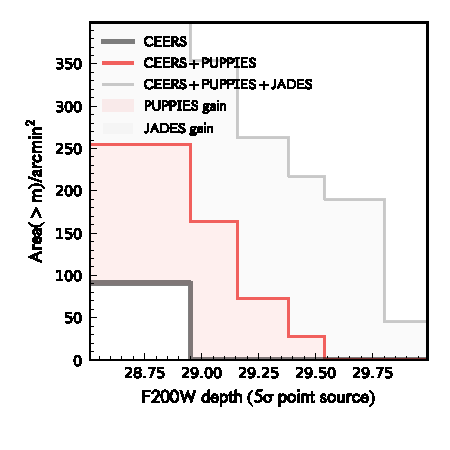
\includegraphics[width=0.6\textwidth]{figs/F200W.pdf}
      \caption{\protect\rule{0ex}{5ex} The cumulative area probed by PUPPIES, JADES, and CEERS, as a function of the F200W depths. \textbf{PUPPIES extends the depth and area of public NIRCam imaging.}}
      \label{fig:depth}
\end{SCfigure}



\begin{figure}[h!]
    \centering
    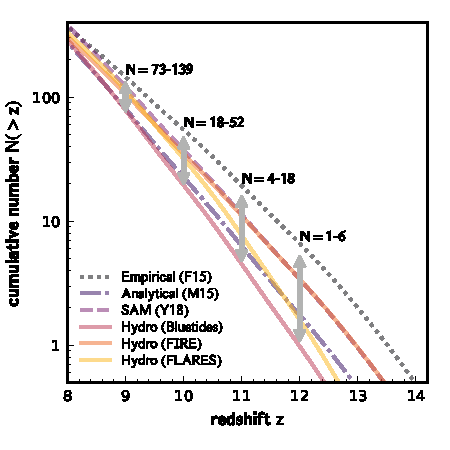
\includegraphics[width=0.49\textwidth]{figs/CN_models.pdf}
    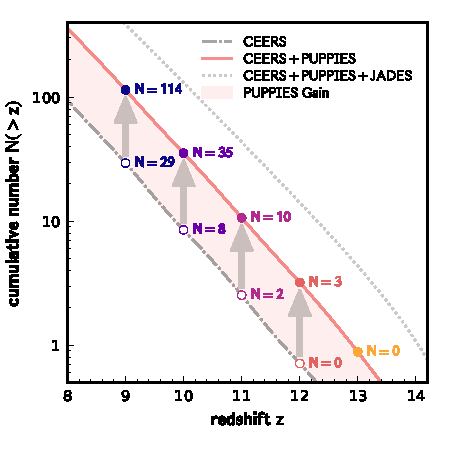
\includegraphics[width=0.49\textwidth]{figs/CN_surveys.pdf}
    \vspace{-5mm}
    \caption{\emph{\underline{Left:}} The cumulative number of galaxies predicted to be accessible to PUPPIES and CEERS for a range of different empirical extrapolations and theoretical models. \textbf{The expected number of galaxies at $z>9$ is uncertain demonstrating the constraining power of PUPPIES. PUPPIES will identify $70-140$ galaxies at $z>9$ and $4-18$ at $z>11$.} \emph{\underline{Right:}} The cumulative number of sources predicted to observable to CEERS, CEERS+PUPPIES, and CEERS+PUPPIES+JADES. \textbf{PUPPIES will boost the number of galaxies at $z>9$ ($z>11$) by a factor of $4$ (5) compared to CEERS alone}. }
    \label{fig:CN}
\end{figure}


\begin{figure}[h!]
    \centering
    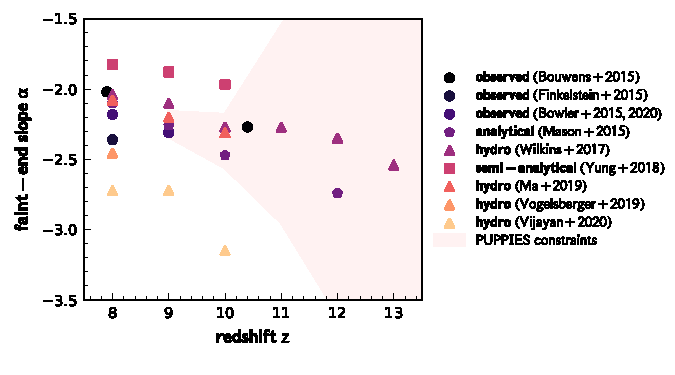
\includegraphics[width=0.8\textwidth]{figs/alpha.pdf}
    \vspace{-5mm}
    \caption{Current observational constraints and theoretical predictions for the faint-end slope $\alpha$ of the luminosity function at $z\ge 8$ alongside forecasts for constraints from PUPPIES + CEERS. \textbf{Predictions for the faint-end slope of the luminosity function $\alpha$ at $z=8-13$ are highly variable. PUPPIES will provide the first meaningful constraints at $z>8$.}}
    \label{fig:alpha}
\end{figure}


\begin{SCfigure}[][h!]
    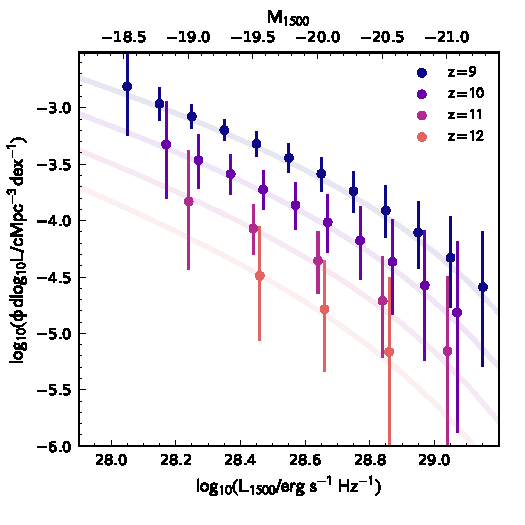
\includegraphics[width=0.6\textwidth]{figs/LF_evo.pdf}
      \caption{\protect\rule{0ex}{10ex} Predicted constraints on the UV luminosity function from PUPPIES at $z=9\to 12$ assuming the Yung et al. (2018) semi-analytical model. \textbf{PUPPIES will enable the first robust constraints on the UV luminosity function at $z>11$.}}
      \vspace{-5mm}
\end{SCfigure}





Compounding the small number of sources is the fact that these programmes, as predominantly contiguous surveys, will suffer from cosmic variance increasing the uncertainty on the number of galaxies by $\approx 1.5-2\times$ compared to the statistical uncertainty alone\cite{2020MNRAS.499.2401T}\cite{2020MNRAS.496..754B}\cite{2008ApJ...676..767T}. 

[{\bf paragraph below needs to be updated for PUPPIES}]



\subsection*{\bf \underline{The Physical Properties of the First Galaxies}}

\subsubsection*{\bf Early Enrichment with Metals and Dust}\label{sec:properties}

As we look back towards the Big Bang the galaxies we discover become increasingly deficient in metals and dust. Exactly when and how the first galaxies became enriched with metals is key outstanding questions in galaxy formation and evolution.

While accurate measurements of the gas and stellar phase metallicities require deep rest-frame optical spectroscopy we can gain the first hints from photometry alone, specifically from the UV continuum slope $\beta$,  where $f_{\lambda}\propto\lambda^{\beta}$. Extremely blue ($\beta = -3$) slopes are only realised for extremely metal poor and dust free stellar populations. The robust identification of galaxies with such slopes will, for the first time, provide the first glimpse into virtually metal-free stellar populations. More generally the UV continuum slope, at least for young star forming galaxies, is sensitive to dust attenuation, itself a tracer of metal enrichment. Thus, while the discovery of galaxies with extremely blue slopes will be exciting, similarly the discovery of galaxies with red $\beta > -2$ provides useful observational constraints on the process of metal and dust enrichment in the early Universe. 

At present, constraints with \emph{Hubble} are effectively limited to $z\sim 7$. Even there $\beta$ is only constrained with a single colour probing only a relatively narrow wavelength range leading to large uncertainties. While it is possible to measure $\beta$ at $9<z<11$ by combining {\em Hubble} and {\em Spitzer} observations \citep[e.g][]{2016MNRAS.455..659W} this relies on the significantly shallower, and often confused, {\em Spitzer} imaging resulting in much larger uncertainties. With our fiducial 6-band strategy we will be able to, for the first time, to \emph{consistently} $\beta$ across the entire reionisation epoch $6<z<12$.

\subsubsection*{\bf Stellar populations}\label{sec:properties}

In addition to $\beta$ PUPPIES will also obtain F444W photometry, probing beyond the Balmer-break at $9<z<11$. This is essential - see technical justification - to measure stellar masses, and thus constrain the galaxy stellar mass function and stellar mass - specific star formation rate relation. With PUPPIES we will measure the galaxy stellar mass function at $z>9$, and where ancillary optical observations are available, at $z<9$. 


\subsubsection{\bf Resolved Structures}

The resolved structures of galaxies encodes information about their structural properties and formation histories and are key observables that can be compared to galaxy formation models.  However we know next to nothing about these properties of $z > 9$ galaxies even though this type of analysis has proven very benefical at lower redshifts (e.g., Mortlock et al. 2013).  Morphologies are also an important assumption used in the measurement of the luminosity function (reference) and only by simultaneously modelling the morphologies, redshifts, and fluxes is it possible to self-consistently measure the luminosity function and its uncertainties. Leveraging NIRCam's resolution we will provide sizes and morphologies of $9<z<11$ galaxies across the rest-frame UV ($0.1-0.4\mu$m).  As can be seen in Fig. \ref{fig:sizes} we will be able too determine structural properties many galaxies.

\begin{SCfigure}[][!h]
    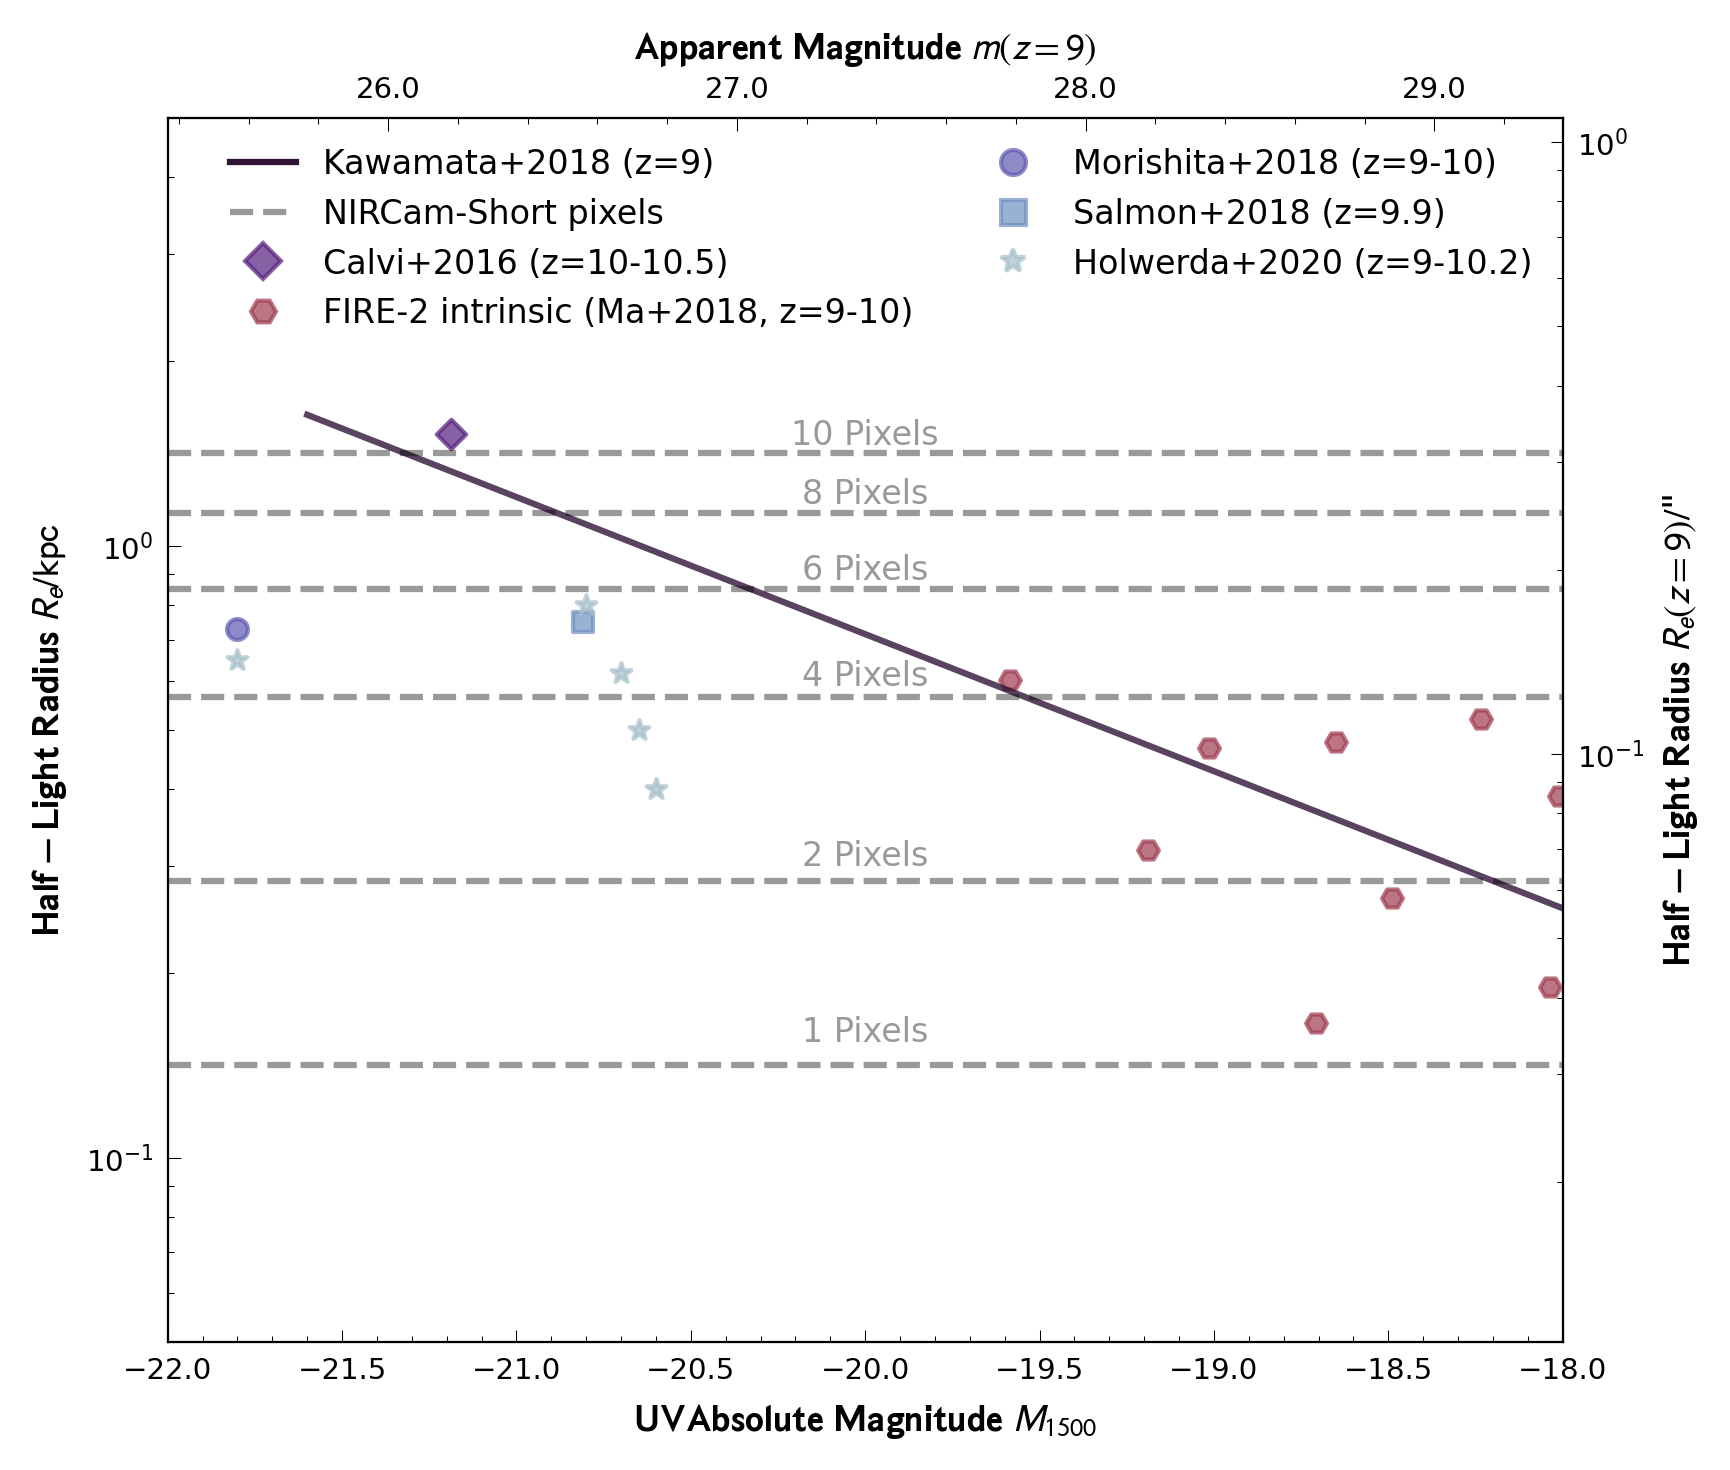
\includegraphics[width=0.6\textwidth]{figs/morph.png}
      \caption{\protect\rule{0ex}{10ex} Current observation constraints and theoretical predictions for the sizes of galaxies at $z>9$. \textbf{Even in under-sampled imaging many $z>9$ galaxies are expected to be resolved in the NIRCam imaging.}}
      \label{fig:sizes}
\end{SCfigure}


What we do know is that massive galaxies at $z < 6$ are often very compact and evolve into red nuggets that have extenguished their star formation a few Gyr after the big bang.  What we do not know is how this occurred.  This is such that these quenched passive ‘red nuggets’ are up to five times smaller at z~3-6 than galaxies of the same mass today.  Since these are certainly the progenitors of modern massive galaxies, studying the ancestors of these compact passive/red galaxies at even higher redshifts is crucial for deciphering their origin.   What we can answer this PUPPIES data is how these early galaxies first formed -- were they large star forming systems that later become compact through some process (Barro et al. 2013; Tacchella et al. 2016)? Or, did these systems formed as compact systems to begin with (e.g., Lilly & Carollo 2016)?   Because our parallel imaging will find the most massive systems, and therefore the progentiors of these passive galaxies, we can answer this question by measuring the sizes of these galaxies.

Related to this is that it is clear that merging activity is very important for distant galaxies up to $z \sim 6$ and likely is even more important at higher redshifts.  The evolution of the density of matter at these early phases of the universe goes as $\sim (1+z)^{3}$, implying that galaxies at $z > 9$ were in a more denser universe than at later times. This implies that the merger rate should be even higher than what we can measure at $z < 6$ with HST.  Duncan et al. (2019) showed that $\sim 40$\% of massive galaxies at $z \sim 6$ are in pairs, with an inferred merger rate of $\sim 10$ mergers Gyr$^{-1}$.  In hierarchical models of galaxy formation these galaxies should be undergone intense merging, which is something that we are directly detect. It is ideal to test this with massive systems which are the easiest observational to find mergers for, given that the secondary system in a pair can be over a magnitude fainter for major mergers.  If we extrapolate the merger fraction history that we can measure at $z > 6$ we find that there should be over 60\% of galaxies in pairs.  This is also a prediction of models such as Illustris and Eagle, which we can test at this high density region of the early universe.  Given that we will detect XX galaxies, our shot noise will produce a merger fraction which is less than 10\% on this measurement.  




\subsection{\bf \underline{Legacy science}}

{\bf could add quiescent galaxies at $z>3$ here}

{\bf -- similar to WAFLS --}

{\bf faint late-type stars}

{\bf faint lower redshift galaxies -- photo-z, physical properties, morphologies}

{\bf follow-up studies}




%%%%%%%%%%%%%%%%%%%%%%%%%%%%%%%%%%%%%%%%%%%%%%%%%%%%%%%%%%%%%%%%%%%%%%%%%%%

%   2. TECHNICAL JUSTIFICATION
%       (see https://jwst-docs.stsci.edu/jwst-opportunities-and-policies/jwst-call-for-proposals-for-cycle-1/jwst-cycle-1-proposal-preparation)
%
%

\clearpage

\justifyobservations   % Do not delete this command.
% Enter your description of the observations.

In this section we justify our choices of survey parameters including the choice of filters, depth, and area, and assess the potential available pure parallel observing opportunities.

\vspace{5mm}
\noindent
\underline{\bf Filter choice: photometric redshifts -- } Simulations show that the combination of 3 filter pairs: {\bf F115W}, {\bf F150W}, {\bf F200W}, {\bf F277W}, {\bf F356W}, and {\bf F444W} is the optimum choice for \emph{robustly} identifying $z>9$ star forming galaxies. As shown in Fig. \ref{fig:s_f} a simple pair of flux-ratios (or color-colour) selection can be used to identify $9<z<11$ galaxies with high completeness and low-contamination. One disadvantage of this approach however is relatively large scatter in the redshifts of individual galaxies resulting in large uncertainties on individual luminosities. A 3-pair photometric redshift selection yield smaller uncertainties on the redshifts and luminosities of individual galaxies and further serves to reduce contamination to $<5\%$.

\begin{SCfigure}[][!h]
    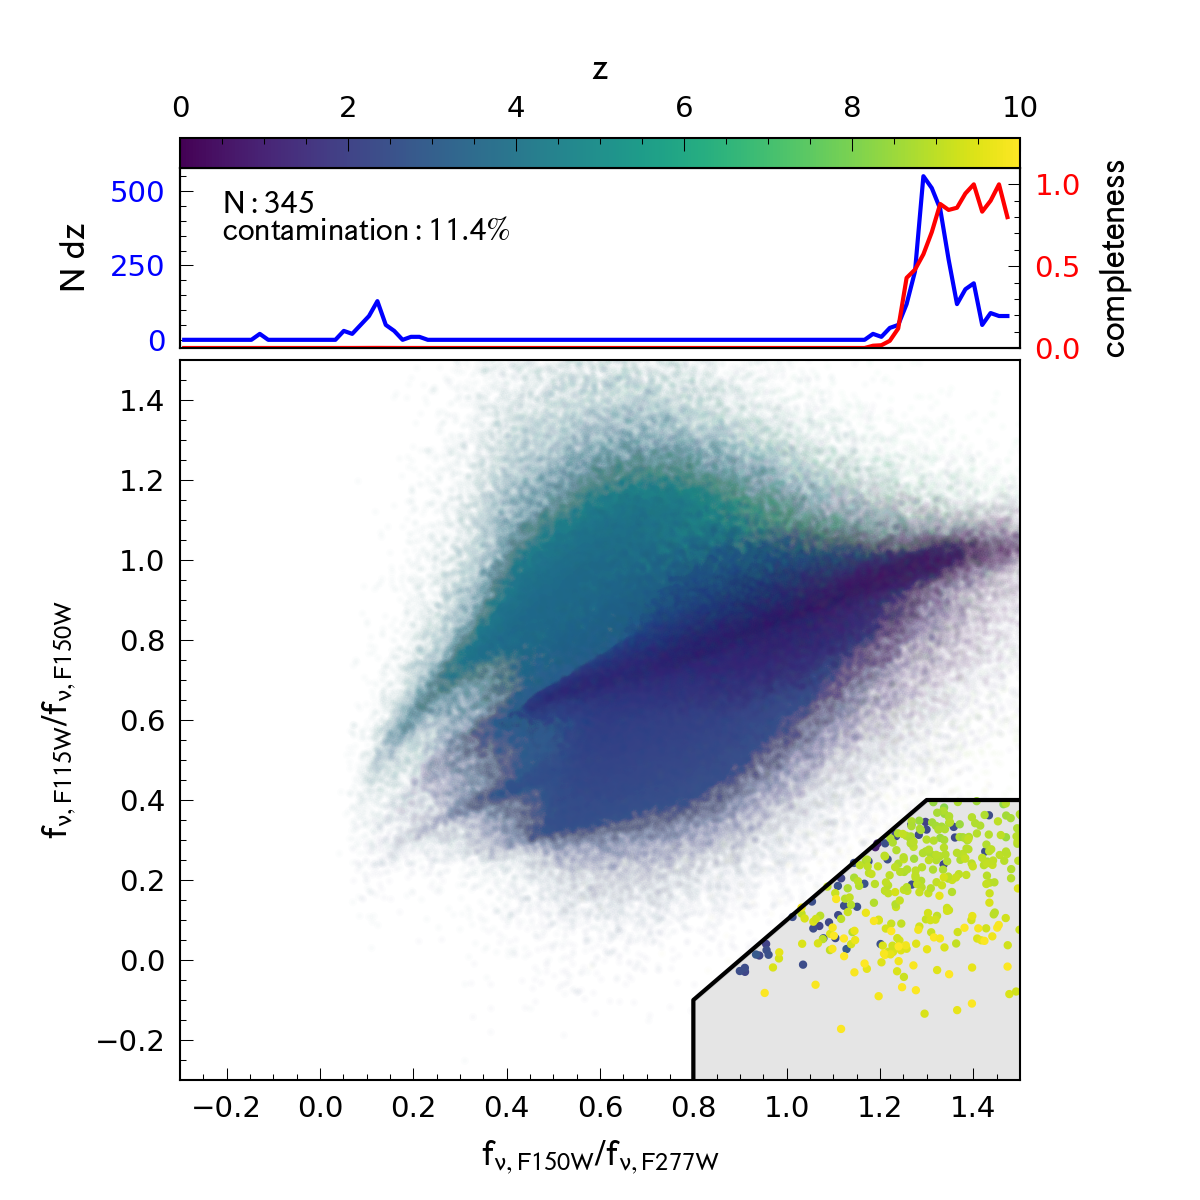
\includegraphics[width=0.6\textwidth]{figs/s_f_F115W.png}
      \caption{\protect\rule{0ex}{10ex} The flux analogue of a colour-colour selection for $9<z<11$ galaxies. Using a mock catalogue from \citet{} combined with photometric noise consistent with our middle tier we demonstrate that a simple pair of flux ratios (or colours) can be used to efficiently select galaxies at $9<z<11$ with contamination $\sim 10\%$ and high-completeness. Sources are only included if they are detected in F277W$>7\sigma$.}
      \label{fig:s_f}
\end{SCfigure}

\noindent
\underline{\bf Filter choice: physical properties -- } Constraining the chemical and dust enrichment of galaxies at $9<z<11$ requires that we probe the rest-frame UV continuum with at least a single colour, and ideally with several bands providing a consistent measurement of the same wavelength range across several redshifts. As demonstrated in Fig. \ref{fig:SED} a 6-band strategy is ideal in this respect as it allows the UV continuum to probed with 3 bands uncontaminated by the Lyman-$\alpha$ and Balmer breaks, encompassing the entire rest-frame UV, across our entire target redshift range. A 4-band strategy allows the measurement of the slope albeit with only a pair of filters uncontaminated by the break.

\vspace{5mm}
\noindent
\underline{\bf Filter choice: alternative strategies -- } While we note that 3 filter pair strategy best matches our scientific objectives these can be partially met using a 2-pair strategy. To keep PUPPIES as flexible as possible in this respect we can also make use of opportunities better suited to a 2-pair strategy.

\begin{figure}[h!]
    \centering
    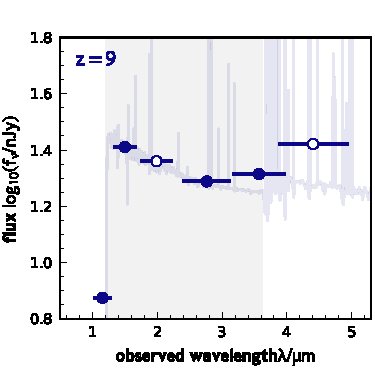
\includegraphics[width=0.3\textwidth]{figs/SED_9.pdf}
    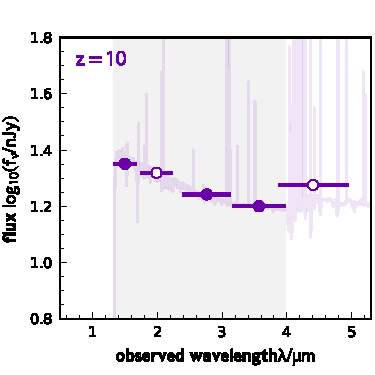
\includegraphics[width=0.3\textwidth]{figs/SED_10.pdf}
    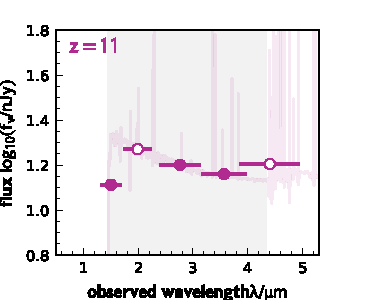
\includegraphics[width=0.3\textwidth]{figs/SED_11.pdf}
    \caption{The model spectral energy distribution and NIRCam fluxes of a star forming galaxy at $z=9$, $10$, and $11$. The shaded area denotes the rest-frame UV continuum between the Lyman-$\alpha$ and Balmer breaks. The alternative 4-band strategy is denoted by the filled symbols. \textbf{The 6-band PUPPIES strategy allows the consistent measurement of the UV continuum slope across the entire UV continuum and redshift range. An alternative 4-band strategy allows the measurement of the slope albeit with a pair of filters uncontaminated by the break. The 6-band strategy also allows us to measure a single band beyond the Balmer-break, essential for measuring stellar masses.}}
    \label{fig:SED}
\end{figure}

The strength of the rest-frame UV - optical colour is a well established diagnostic of the recent star formation activity in galaxies. However, the colour is also sensitive to dust attenuation and thus, in the absence of additional constraints, the UV - optical colour is degenerate. However, the UV continuum slope $\beta$ is a well established diagnostic of dust attenuation: redder galaxies are generally dustier. Combining these two diagnostics then allows us to constrain both the dust attenuation and the specific star formation rate. This is demonstrated in  Fig. \ref{fig:beta} where simulation galaxies, from the FLARES project \citep{2020MNRAS.tmp.3168L}, are shown in the $\beta$ and F356W-F444W plane and colour coded by $A_{1500}$ (left) and specific star formation rate (right). At fixed $\beta$ F356W-F444W is correlated with specific star formation rate. For fields observed with our 6-band strategy PUPPIES will enable the measurement of the stellar masses and specific star formation rates.

\begin{figure}[h!]
    \centering
    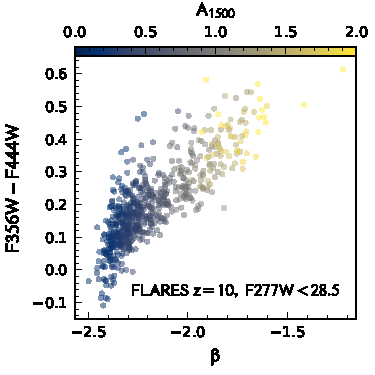
\includegraphics[width=0.45\textwidth]{figs/beta_A1500.pdf}
    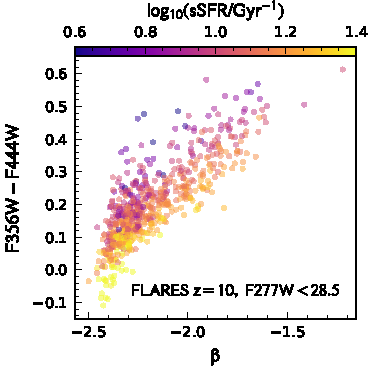
\includegraphics[width=0.45\textwidth]{figs/beta_sSFR.pdf}
    % 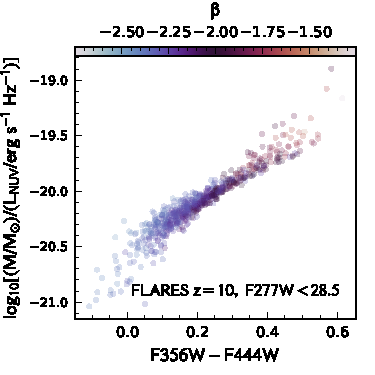
\includegraphics[width=0.3\textwidth]{figs/C_beta_MTOL.pdf}
    \caption{The relationship between $\beta$ and F356W-F444W for simulated galaxies at $z=10$ colour-coded by $A_{1500}$ (\emph{\underline{left}}) and specific star formation rate (\emph{\underline{right}}) predicted by the FLARES simulation (Lovell+2020; Vijayan+2020). At these redshifts $\beta$ is strongly correlated with dust attenuation while at fixed $\beta$ the specific SFR is correlated with F356W$-$F444W. \textbf{The 6 filter observations obtained by PUPPIES will enable us to measure the dust attenuation, total star formation rates, and stellar masses of galaxies at $z>8$.}}
    \label{fig:beta}
\end{figure}

\vspace{5mm}
\noindent
\underline{\bf Area and Depth - } In the absence of cosmic variance, the core science objective of PUPPIES - to constrain the faint-end slope and normalisation of the $9<z<11$ - is best realised by going as deep as possible. This is both because the expected number of galaxies increases faster than $f_{\nu}^2$ due to the steepness of the luminosity function and going deeper extends the luminosity range. Going deeper also provides stronger complementarity with the public $\sim 90\ {\rm arcmin}^2$ CEERS NIRCam imaging. However, a single, or small number of fields, is susceptible to cosmic-variance, which will dominate over the statistical (Poisson) variance \citep[e.g][]{2020MNRAS.499.2401T}. From our analysis, based on the methodology of \citet{2020MNRAS.499.2401T}, a good compromise is afforded by combining $10-20$ pointings with durations $10^4-10^5$s long. 

\vspace{5mm}
\noindent
\underline{\bf Availability of deep NIRCam parallel opportunities - }
To determine the type, and thus potential depth, of opportunities that are available we use the public GTO and ERS APTs and filter out all observations that 1) already have attached coordinated parallels, 2) have the \texttt{NoParallel} flag set, and 3) those of targets with high-background ($>0.3\ {\rm MJy/Sr}$). To estimate the amount of time available to teach unique target we sum the science durations of all observations using the same instrument. The predicted distribution of opportunities with science durations $t_{\rm SD}>10^{4}$ s is then shown in Figure \ref{fig:time_background}: this analysis suggests $\sim 50$ GTO/ERS opportunities with $t_{\rm SD}>10^{4}$ s; assuming this distribution is representative of the final Cycle 1 observation suggests there should be $100-150$ useful opportunities.

\begin{SCfigure}
    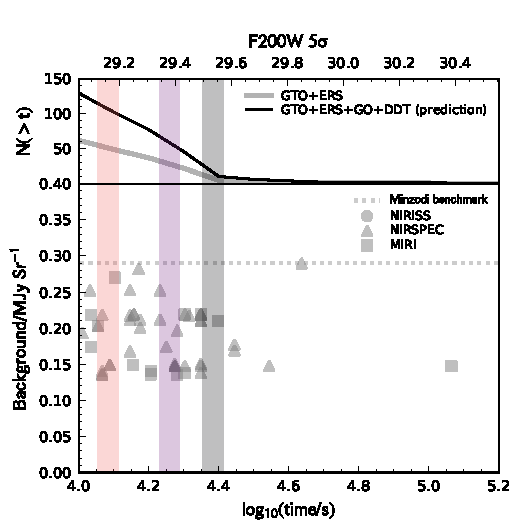
\includegraphics[width=0.6\textwidth]{figs/time_background.pdf}
      \caption{\protect\rule{0ex}{10ex} The predicted distribution of science durations $t_{\rm SD}$ and backgrounds for pure parallel observing opportunities based on the existing GTO and ERS programs. The vertical bands denote the 3 tiers used to define our fiducial survey while the horizontal lines denote the $2\mu$m \texttt{minzodi} benchmark background and the minimum background in several deep extragalactic fields. The top panel shows the resulting cumulative distribution of opportunities as well as an extrapolation to the full cycle 1 observations.}
      \label{fig:time_background}
\end{SCfigure}

\vspace{5mm}
\noindent
\underline{\bf Fiducial programme:} Armed with this knowledge of the predicted number and distribution of available parallel opportunities we define a fiducial programme consisting of three tiers - ABC - assuming 4, 3, and 2 \texttt{deep8} 10 group exposures respectively. Reflecting the greater availability of shorter duration opportunities we choose, for this fiducial programme, to obtain 3, 5, and 10 pointings for the A, B, and C tiers respectively. The resulting area and depths achieved in each tier are summarised below. \textbf{The total exposure time as reported by the APT for the combination of the 3 tiers is 79.3 hours}. This fiducial programme serves only to demonstrate what should be possible with a PUPPIES-\emph{like} programme and not a firm requirement.

\begin{table}[h!]
\footnotesize
\begin{center}
\begin{tabular}{ |c|c|c|c|c|c|c|c|c| } 
\hline
\multicolumn{3}{|c|}{} & \multicolumn{6}{|c|}{$5\sigma$ point-source depth} \\
 \hline
Tier & $N_{p}$ & Area$/{\rm arcmin^2}$ & F115W & F150W & F200W & F277W & F356W & F444W \\
\hline
\textbf{A} & 3 & 27 & 29.19 & 29.37 & 29.54 & 29.09 & 29.15 & 28.86 \\
\textbf{B} & 5 & 45 & 29.03 & 29.22 & 29.38 & 28.94 & 28.99 & 28.70 \\
\textbf{C} & 10 & 91 & 28.81 & 28.99 & 29.16 & 28.71 & 28.77 & 28.48 \\
\hline
\end{tabular}
\end{center}
\vspace{-5mm}
\caption{The number of pointings $N_p$, area, and 5$\sigma$ point source depths in each filter for our 3 tiers for our fiducial survey.  Depths assume a short-wavelength (long-wavelength) apertures of $0.08$" ($0.16$"), background at the benchmark level of the \texttt{Minzodi} location as defined by \texttt{Pandeia}. The ABC tiers assume 4, 3, 2 exposures of 10 groups assuming the \texttt{DEEP8} readout mode respectively.}
\end{table}

\vspace{5mm}
\noindent
\underline{\bf Preferred distribution and flexibility - } While 
This fiducial programme defined above serves only to demonstrate what should be possible with a PUPPIES-\emph{like} programme and not a firm requirement. Within the confines of our requirement for 10-20 deep (F200W$>29$), low-background, independent pointings we are flexible in our choice observing opportunities. We will however seek to obtain a balanced programme mixing deeper and shallower opportunities. Where possible we will also express a preference for targets with meaningful existing ancillary observations and accessible to the Southern Hemisphere.

%%%%%%%%%%%%%%%%%%%%%%%%%%%%%%%%%%%%%%%%%%%%%%%%%%%%%%%%%%%%%%%%%%%%%%%%%%%

%   3. SPECIAL REQUIREMENTS
%        (see https://jwst-docs.stsci.edu/jwst-opportunities-and-policies/jwst-call-for-proposals-for-cycle-1/jwst-cycle-1-proposal-preparation)
%
%
\specialreq             % Do not delete this command.
% Justify your special requirements here, if any.

%%%%%%%%%%%%%%%%%%%%%%%%%%%%%%%%%%%%%%%%%%%%%%%%%%%%%%%%%%%%%%%%%%%%%%%%%%%

%   4. COORDINATED PARALLEL OBSERVATIONS
%        (see https://jwst-docs.stsci.edu/jwst-opportunities-and-policies/jwst-call-for-proposals-for-cycle-1/jwst-cycle-1-proposal-preparation)
%
%
\coordinatedobs % Do not delete this command.
% Enter your coordinated parallel observing plans here, if any.

%%%%%%%%%%%%%%%%%%%%%%%%%%%%%%%%%%%%%%%%%%%%%%%%%%%%%%%%%%%%%%%%%%%%%%%%%%%

%   5. JUSTIFY DUPLICATIONS
%        (see https://jwst-docs.stsci.edu/jwst-opportunities-and-policies/jwst-call-for-proposals-for-cycle-1/jwst-cycle-1-proposal-preparation)
%
%
\duplications           % Do not delete this command.
% Enter your duplication justifications here, if any.

%%%%%%%%%%%%%%%%%%%%%%%%%%%%%%%%%%%%%%%%%%%%%%%%%%%%%%%%%%%%%%%%%%%%%%%%%%%

%   6. ANALYSIS PLAN
%       (see https://jwst-docs.stsci.edu/jwst-opportunities-and-policies/jwst-call-for-proposals-for-cycle-1/jwst-cycle-1-proposal-preparation)
%
%
\analysisplan % Do not delete this command.
% Describe the data processing and analysis plan here.

%%%%%%%%%%%%%%%%%%%%%%%%%%%%%%%%%%%%%%%%%%%%%%%%%%%%%%%%%%%%%%%%%%%%%%%%%%%

\clearpage

\bibliography{PUPPIES}


\end{document}          % End of proposal. Do not delete this line.
                        % Everything after this command is ignored.
